\subsection{Composite Design Pattern}

	\defn{Composite Design}{is one of the structural design patterns, which is used when one is concerned with representing \ita{part-whole} hierarchies as tree structures}

	\rem{clients can treat indivisual objects and their compositions in the same way}

	\par{The key idea here is to have a common abstract classs - \ita{component} - that represents both primitive objects - \ita{leaf} - and their aggregated container objects - \ita{composite}.}

	\defn{Leaf}{ defines behaviour for primitive objects, hence it has no children}

	\defn{Component}{ is the abstract class which \ita{declares} the interface for objects in the composition, implements default behaviour and declares an interface for accessing all managed child components}

	\defn{Composite}{ defines behaviour for objects with children, stores child components and \ita{implements} operations defined by \texttt{Component}}

	\subsubseciton{Applicability}

		\par{The Composite pattern is applicable when:}

		\begin{itemize}
			\item part-whole hierarchies need to be represented as objects
			\item the differences between objects and their compositions are irrelevant
		\end{itemize}

	\subsubsection{Structure}

		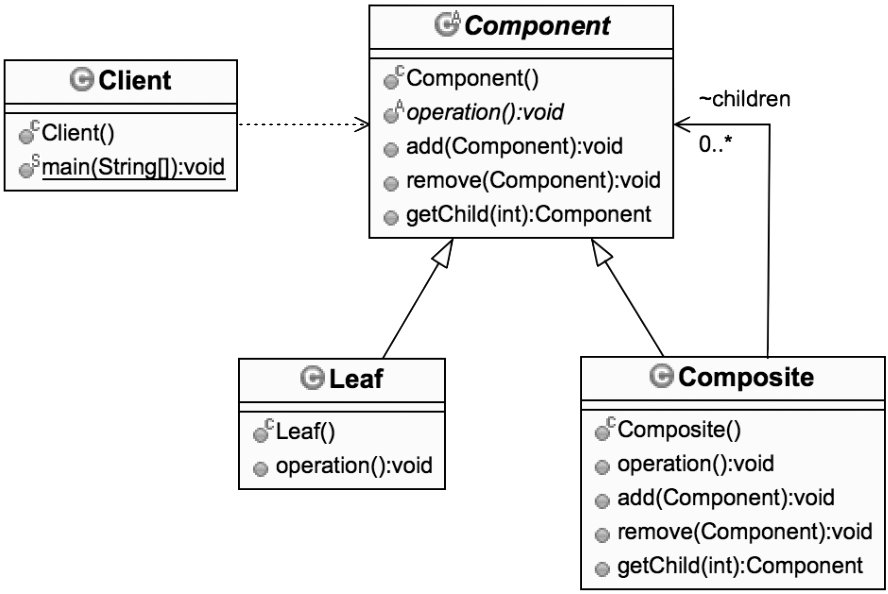
\includegraphics{pattern_composite}
		% without pattern
		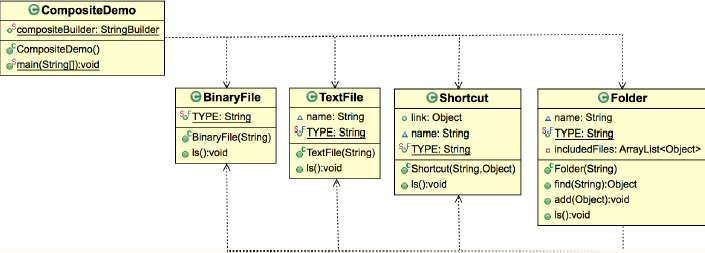
\includegraphics{pattern_composite2}
		% refactores using pattern
		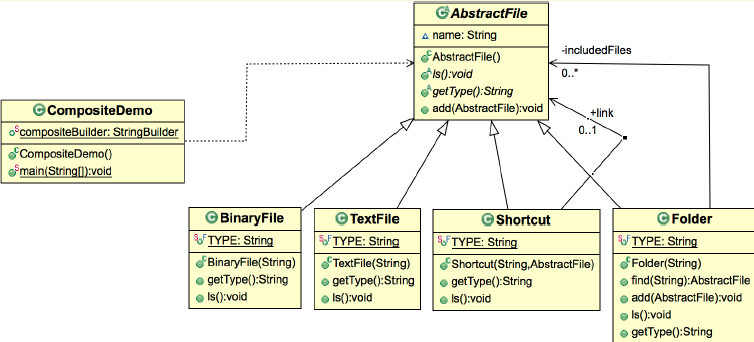
\includegraphics{pattern_composite3}

		\par{Note how in the first implementation we must first query the type of the object before calling \texttt{ls()}, and adding a new component would mean updating all toher classes}

		\rem{note how composite beahviour is \texttt{void} in superclass and is left to be implemented in each leaf}

		\rem{component must be abstract since if using an interface, then variables of type \texttt{final} (e.g. name) would be defined at the superclass level, and would all be the same for all children (i.e all files would need to have the same name)}



	\subsubsection{Summary}

		\begin{itemize}
			\item structural
			\item concerned with how classes and objects are composed to form larger structures
			\item helps representing part-whole hierarchies into tree structures composed of objects
		\end{itemize}

		
